\chapter{Boot Overview \label{regboot}}


\section {SDM660 Chip Set Overview}

为了接下来更好的理解启动流程,图\ref{chipset}\footnote[1]{摘自SDM630/SDA630 Device Specification}是SMD660 的Chipset, 
我们可以从中提取出 启动系统必须的 Processor, Memory:
\begin{figure*}[htbp]
\begin{center}
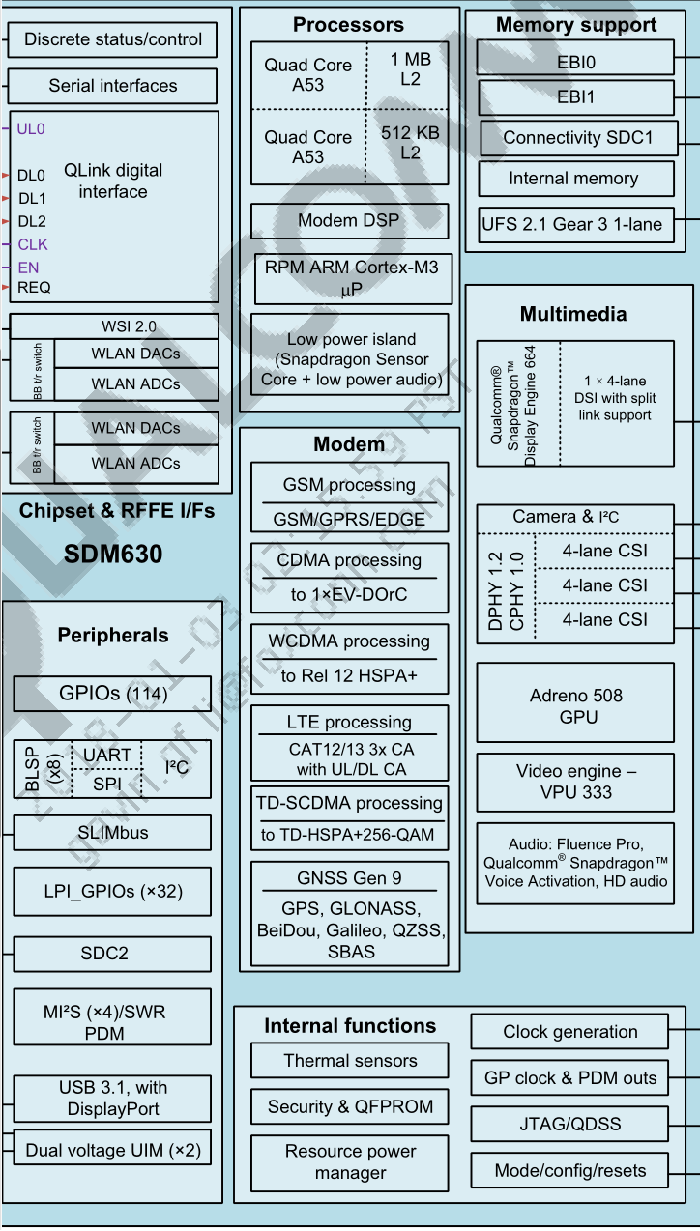
\includegraphics[width=13cm]{img/sdm660arch}
\caption{SDM660 chipset}
\label{chipset}
\end{center}
\vspace{-0.5em}
\end{figure*}

\begin{itemize}

\item Processors

\begin{itemize}


\item Application Processor

Arm V8 架构(指令集)的Cortex-A53,寻址范围是64bit, octa core subsystem.
其中:
\begin{itemize}
\item 四个 high-performance(高性能) ARM Cortex-A53 cores 可以运行在 2.2 GHz, 有 1 MB L2 cache(二级缓冲)。

\item 四个 low-power(低功耗)的 A53 ,运行在 1.843 GHz,他们有着 512KB L2 cache(二级缓冲)。
\end{itemize}

\item Modem, 使用的是Qualcomm ® Hexagon™ DSP V61H 1 GHz 1.5 MB L2 caches; DSDS 。注意到DSP ,应该是数字信号处理。

\item RPM system,Cortex-M3,Resource Power Manager(资源功耗管理)。

\item Low-power island.Low-power island with Hexagon DSP consists of Snapdragon sensor core and
low-power audio subsystem

\end{itemize}

\item Memory

\begin{itemize}

\item EBI(External Bus Interface),一种内存控制接口。意义是,可以使不同的内存控制器,使用
同一套 数据和地址 Pin set. SDM660 有 双通道,高速(1333Mhz)LPDDR4X SDRAM.

\item 其他的 

256 KB IMEM 

136 KB GMEM for graphics

512 KB VMEM for video

TCM


\item 储存

UFS 2.1 gear 3 (one-lane),eMMC 5.1, SD 3.0。



1) APPS PBL; 2) XBL; 3) RPM; 4) APPS SBL; 5) HLOS; 6) modem PBL;
7) SP PBL


\end{itemize}



\end{itemize}






\section {SDM660 boot Overview}


这里对SDM660的启动流程做一些讨论。




根据

\begin{figure*}[htbp]
\begin{center}
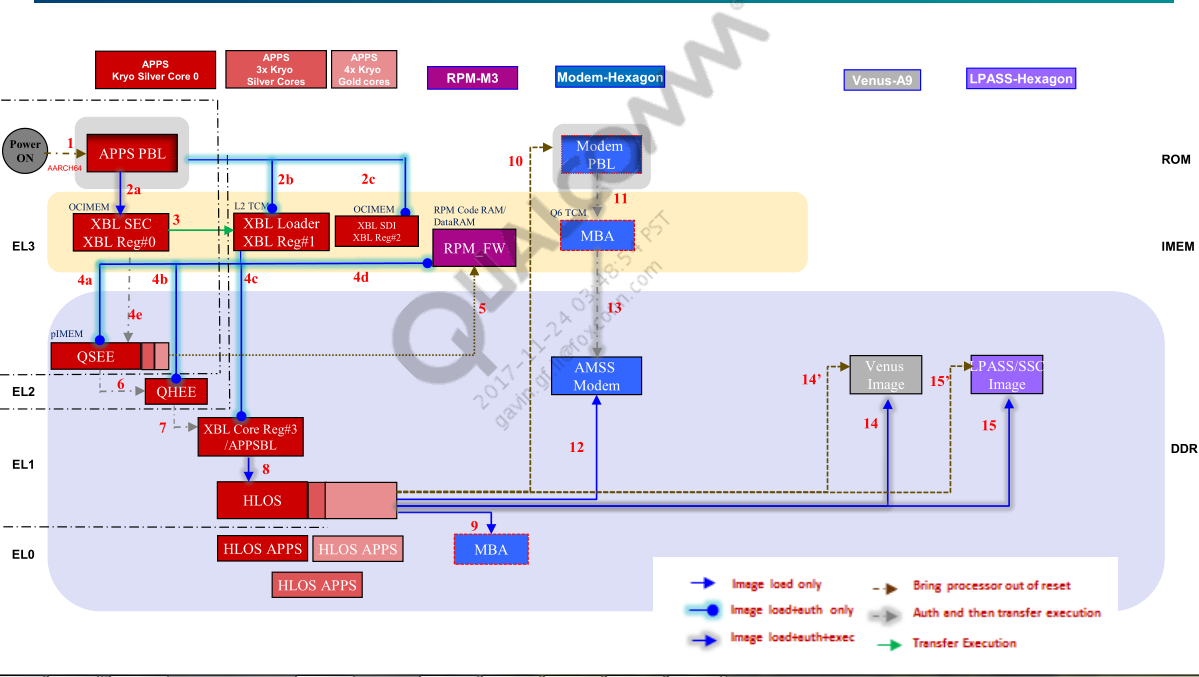
\includegraphics[width=16cm]{img/bootarch}
\caption{SDM660 boot flow}
\label{sdm660boot}
\end{center}
\vspace{-0.5em}
\end{figure*}




\begin{itemize}

\item APPS PBL
APPS cpu core0 从rom 里加载执行 PBL .

主要动作有: 建立APPS根信任环境( RoT),decryption  XBL Loader,探测boot 设备,支持Emergency Download。
加载 xbl 到 OCIMEM ,L2TCM,RPM CodeRAM.

\begin{itemize}
\item a. Loads and authenticates XBL SEC (region \#0) from the storage device to OCIMEM.
\item  b. Loads and authenticates XBL loader (region \#1) from the storage device to L2TCM.
\item c. Loads and authenticates XBL ramdump (region \#2) to OCIMEM, then jumps to XBL region \#1.
\end{itemize}

\item xbl

\begin{itemize}
\item xbl sec在EL3 进行安全方面的配置,然后执行xbl 其他部分。
\item  b. Loads and authenticates XBL loader (region \#1) from the storage device to L2TCM.
\item c. Loads and authenticates XBL ramdump (region \#2) to OCIMEM, then jumps to XBL region \#1.
\end{itemize}


\item  

\item 

\end{itemize}




\section{附录 一. xbl loader info\label{loaderinfo}}



\begin{lstlisting}
re Boot: Off
S - Boot Config @ 0x00786070 = 0x000001c1
S - JTAG ID @ 0x00786130 = 0x000ac0e1
S - OEM ID @ 0x00786138 = 0x00000000
S - Serial Number @ 0x00784138 = 0xcd2bcd5b
S - OEM Config Row 0 @ 0x00784188 = 0x0000000000000000
S - OEM Config Row 1 @ 0x00784190 = 0x0000000000000000
S - Feature Config Row 0 @ 0x007841a0 = 0x0070302012400300
S - Feature Config Row 1 @ 0x007841a8 = 0x0000000000000820
S - Core 0 Frequency, 3952 MHz
S - PBL Patch Ver: 4
S - I-cache: On
S - D-cache: On


/*@brief
*   This funcion will parse the PBL timestamp milestones passed to SBL
*   and insert them into the boot log.  Currently PBL's unit of measure is
*   clock ticks.  PBL does not pass the clock frequency yet so it is hard
*   wired to 19.2 Mhz.  Also PBL does not pass the names of each field so for
*   now reference a structure of our own to get the names which will have
*   logic ready for the day PBL starts passing them.
*/
void boot_pbl_log_milestones(boot_pbl_shared_data_type * pbl_shared_data)
{
	...
  for (count = 0;count < (sizeof(pbl_shared_data->timestamps) / sizeof(uint32));count++, pbl_timestamp++)
  {
    pbl_us_value = ( ( (uint64)(*pbl_timestamp) ) * PS_PER_PBL_TIMESTAMP_TICK ) / 1000000;
    /*Logs message and time. */
    boot_log_message_raw(boot_log_pbl_milestone_names[count],(uint32)pbl_us_value,LOG_MSG_TYPE_BOOT,NULL);
  }
	...
}
B -         0 - PBL, Start
B -      7114 - bootable_media_detect_entry, Start
B -    135758 - bootable_media_detect_success, Start
B -    135764 - elf_loader_entry, Start
B -    137445 - auth_hash_seg_entry, Start
B -    137780 - auth_hash_seg_exit, Start
B -    189261 - elf_segs_hash_verify_entry, Start
B -    238916 - elf_segs_hash_verify_exit, Start
B -    238929 - auth_xbl_sec_hash_seg_entry, Start
B -    268084 - auth_xbl_sec_hash_seg_exit, Start
B -    268086 - xbl_sec_segs_hash_verify_entry, Start
B -    274847 - xbl_sec_segs_hash_verify_exit, Start
B -    274894 - PBL, End




sbl1_boot_logger_init

B -    301340 - SBL1, Start
B -    304664 - usb: hs_phy_nondrive_start
B -    305000 - usb: hs_phy_nondrive_finish
B -    305030 - boot_flash_init, Start
D -        30 - boot_flash_init, Delta
B -    305061 - sbl1_ddr_set_default_params, Start
D -       152 - sbl1_ddr_set_default_params, Delta
B -    305213 - boot_config_data_table_init, Start
B -    324825 - Using default CDT
D -     19611 - boot_config_data_table_init, Delta - (0 Bytes)
B -    324855 - CDT Version:3,Platform ID:8,Major ID:1,Minor ID:0,Subtype:0

boot_config_process_entry
B -    324855 - Image Load, Start

boot_auth_image_hashtable-> boot_sec_img_auth_verify_metadata
D -       671 - Auth Metadata
D -       458 - Segments hash check

D -      4972 - PMIC Image Loaded, Delta - (34272 Bytes)

sbl1_config_table 中有load_apdp_image_pre_procs
加载时要预先执行的函数列表
boot_procedure_func_type load_apdp_image_pre_procs[] = 
{
  /* Initialize PMIC and railway driver */
  sbl1_hw_pre_ddr_init,

B -    329827 - pm_device_init, Start
B -    331596 - PM: 0x1210: 00
B -    331596 - PM: battery present
B -    332114 - PM: PON REASON: PM0=0x8000028000000001:0x0 PM1=0x8000088000000020:0x0 
B -    372984 - PM: SET_VAL:Skip
D -     44072 - pm_device_init, Delta
B -    373899 - pm_driver_init, Start
B -    377620 - PM: OCP Clearing for L4A is Skipped :PM660 is not supported the LDO4
D -      4056 - pm_driver_init, Delta
B -    377956 - pm_sbl_chg_init, Start
B -    380182 - PM: Trigger FG IMA Reset
B -    380396 - PM: Trigger FG IMA Reset.Completed
B -    381677 - PM: EntryVbat: 4313; EntrySOC: -1
B -    381768 - PM: BATT TEMP: 28 DegC
D -      3995 - pm_sbl_chg_init, Delta
B -    381982 - vsense_init, Start
D -         0 - vsense_init, Delta


APDP Image Loaded
	sbl1_ddr_set_params,

B -    429623 - Pre_DDR_clock_init, Start
D -       396 - Pre_DDR_clock_init, Delta
D -         0 - sbl1_ddr_set_params, Delta

(boot_procedure_func_type)sbl1_ddr_init,
B -    435265 - DSF version = 35.0, DSF RPM version = 22.0
B -    435265 - Max Frequency = 1296 MHz,  platform_id = 0x3007
B -    435387 - do_ddr_training, Start
B -    442341 - Bootup frequency set to 1296000
D -      7045 - do_ddr_training, Delta
B -    457347 - ddr_mfr = 0xff
B -    457347 - ddr_type = 0x7
B -    457378 - ddr_size = 0x1000 MB


sbl1_hw_init_secondary,
B -    469395 - clock_init, Start
D -       305 - clock_init, Delta
}

boot_config_process_entry
sbl1_load_sec_partition

B -    470127 - Image Load, Start
D -         0 - APDP Image Loaded, Delta - (0 Bytes)
B -    470188 - usb: EMMC Serial - af7320
B -    470249 - usb: fedl, vbus_low
B -    472963 - PM: 0: PON=0x1:HARD_RESET: ON=0x80:PON_SEQ: POFF=0x2:PS_HOLD: OFF=0x80:POFF_SEQ
B -    473055 - PM: 1: PON=0x20:PON1: ON=0x80:PON_SEQ: POFF=0x8:GP1: OFF=0x80:POFF_SEQ
B -    473085 - PM: SMEM Chgr Info Write Success
B -    473177 - sbl1_efs_handle_cookies, Start
D -       579 - sbl1_efs_handle_cookies, Delta
B -    473848 - Image Load, Start
D -      2775 - Auth Metadata
D -      1068 - Segments hash check
D -      6527 - QSEE Dev Config Image Loaded, Delta - (42024 Bytes)
B -    480405 - Image Load, Start
D -       518 - SEC Image Loaded, Delta - (4096 Bytes)
B -    480924 - Image Load, Start
D -     21472 - Auth Metadata
D -     18270 - Segments hash check
D -     61762 - QSEE Image Loaded, Delta - (1945112 Bytes)
B -    542717 - Image Load, Start
D -      2776 - Auth Metadata
D -      3050 - Segments hash check
D -     10675 - QHEE Image Loaded, Delta - (273136 Bytes)
B -    553453 - Image Load, Start
D -      2867 - Auth Metadata
D -      2196 - Segments hash check
D -     11407 - RPM Image Loaded, Delta - (219340 Bytes)
B -    565348 - Image Load, Start
D -        30 - STI Image Loaded, Delta - (0 Bytes)
B -    565836 - Image Load, Start
D -      2806 - Auth Metadata
D -      3324 - Segments hash check
D -     11559 - ABL Image Loaded, Delta - (379472 Bytes)
B -    577456 - Image Load, Start
D -      3386 - Auth Metadata
D -     13939 - Segments hash check
D -     29280 - APPSBL Image Loaded, Delta - (1792000 Bytes)
B -    607133 - SBL1, End
D -    305823 - SBL1, Delta
S - Flash Throughput, 80000 KB/s  (4694664 Bytes,  58271 us)
S - DDR Frequency, 1296 MHz
\end{lstlisting}


\section{ 附录 关键代码}


\subsection{boot\_configuration\_table\_entry \label{sbl1_config_table}}
\begin{lstlisting}
typedef struct
{
  image_type host_img_id;                 /**< Image ID of the host */
  config_image_type host_img_type;        /**< Image type of the host */ 
  image_type target_img_id;               /**< Image ID of the target */ 
  config_image_type target_img_type;      /**< Image type of the target */ 
  secboot_sw_type target_img_sec_type;    /**< Secure Software ID of the target */
  boot_boolean load;                      /**< Target will be loaded */
  boot_boolean auth;                      /**< Target will be authenticated */
  boot_boolean exec;                      /**< Target will execute immediately after
                                               loading/authentication */
  boot_boolean jump;                      /**< Target will be jumped to after
                                               post procedures are complete */ 
  boot_procedure_func_type exec_func;     /**< Function pointer to execute function.
                                               Must be defined if exec is TRUE */ 
  boot_procedure_func_type jump_func;     /**< Function pointer to jump function.
                                               Must be defined if jump is TRUE */ 
  boot_procedure_func_type *pre_procs;    /**< Function pointer array to pre-procedures */
  boot_procedure_func_type *post_procs;   /**< Function pointer array to post-procedures */
  boot_logical_func_type boot_load_cancel;/**< Function pointer to cancel loading */ 
  uint8 * target_img_partition_id;        /**< Target image partition ID information */
  uint8 * target_img_str;                  /**< Target image name information  */
  whitelist_region_type * whitelist_table; /**< Whitelist table */
  boot_boolean boot_ssa_enabled;           /**< Subsystem self authentication (ssa)*/
  boot_boolean enable_rollback_protection; /**< Enable Roll back protection feature or not */
  boot_boolean enable_xpu;                 /**< Enable XPU configuration for the image */
  uint32 xpu_proc_id;                      /**< XPU proc id to be passed to TZ */
  uint32 sbl_qsee_interface_index;        /**< Index of this image's entry in sbl qsee interface struct */
  uint64 seg_elf_entry_point;             /**< Entry point for segmented ELF */
  uint32 RESERVED_3;                      /**< RESERVED */
  uint32 RESERVED_4;                      /**< RESERVED */
}boot_configuration_table_entry;




boot_configuration_table_entry sbl1_config_table[] = 
{

  /* SBL1 -> PMIC */
  {
    SBL1_IMG,                   /* host_img_id */
    CONFIG_IMG_QC,              /* host_img_type */
    GEN_IMG,                    /* target_img_id */
    CONFIG_IMG_ELF,             /* target_img_type */
    SECBOOT_PMIC_SW_TYPE,       /* target_img_sec_type */ 
    TRUE,                       /* load */
    TRUE,                       /* auth */
    FALSE,                      /* exec */
    FALSE,                      /* jump */
    NULL,                       /* exec_func */
    NULL,                       /* jump_func */
    load_pmic_pre_procs,        /* pre_procs */ 
    load_pmic_post_procs,       /* post_procs */
    pmic_load_cancel,           /* load_cancel */
    pmic_partition_id,          /* target_img_partition_id */
    (uint8*)PMIC_BOOT_LOG_STR,  /* target_img_str */
    NULL,                       /* whitelist table */
    FALSE,                      /* boot_ssa_enabled */
    TRUE,                       /* enable_rollback_protection*/
    FALSE,                      /* enable_xpu */
    0x0,                        /* xpu_proc_id*/    
    0x0,                        /* sbl_qsee_interface_index */
    0x0                         /* seg_elf_entry_point*/
  },

  /* SBL1 -> APDP */
  {
    SBL1_IMG,                   /* host_img_id */
    CONFIG_IMG_QC,              /* host_img_type */
    GEN_IMG,                    /* target_img_id */
    CONFIG_IMG_ELF,             /* target_img_type */
    SECBOOT_APDP_SW_TYPE,       /* target_img_sec_type */ 
    TRUE,                       /* load */
    TRUE,                       /* auth */
    FALSE,                      /* exec */
    FALSE,                      /* jump */
    NULL,                       /* exec_func */
    NULL,                       /* jump_func */
    load_apdp_image_pre_procs,    /* pre_procs */ 
    load_apdp_image_post_procs,   /* post_procs */
    apdp_load_cancel,           /* load_cancel */
    apdp_partition_id,          /* target_img_partition_id */
    APDP_BOOT_LOG_STR,          /* target_img_str */
    NULL,                       /* whitelist table */
    FALSE,                      /* boot_ssa_enabled */
    TRUE,                       /* enable_rollback_protection*/
    FALSE,                      /* enable_xpu */
    0x0,                        /* xpu_proc_id*/    
    0x0,                        /* sbl_qsee_interface_index */
    0x0                         /* seg_elf_entry_point*/
  },

  /* SBL1 -> Qsee Dev config image  */
  {
    SBL1_IMG,                            /* host_img_id */
    CONFIG_IMG_QC,                       /* host_img_type */
    GEN_IMG,                             /* target_img_id */
    CONFIG_IMG_ELF,                      /* target_img_type */
    SECBOOT_QSEE_DEVCFG_SW_TYPE,         /* target_img_sec_type */ 
    TRUE,                                /* load */
    TRUE,                                /* auth */
    FALSE,                               /* exec */
    FALSE,                               /* jump */
    NULL,                                /* exec_func */
    NULL,                                /* jump_func */
    NULL,                                /* pre_procs */ 
    load_qsee_devcfg_image_post_procs,   /* post_procs */
    qsee_devcfg_image_load_cancel,       /* load_cancel */
    qsee_devcfg_image_partition_id,      /* target_img_partition_id */
    QSEE_DEVCFG_BOOT_LOG_STR,            /* target_img_str */
    NULL,                                /* whitelist table */
    FALSE,                               /* boot_ssa_enabled */
    FALSE,                               /* enable_rollback_protection*/
    FALSE,                               /* enable_xpu */
    0x0,                                 /* xpu_proc_id*/    
    0x0,                                 /* sbl_qsee_interface_index */
    0x0                                  /* seg_elf_entry_point*/
  },  
  
 /* SBL1 -> QSEE */
  {
    SBL1_IMG,                   /* host_img_id */
    CONFIG_IMG_QC,              /* host_img_type */
    GEN_IMG,                    /* target_img_id */
    CONFIG_IMG_ELF,             /* target_img_type */
    SECBOOT_QSEE_SW_TYPE,       /* target_img_sec_type */ 
    TRUE,                       /* load */
    TRUE,                       /* auth */
    FALSE,                      /* exec */
    FALSE,                      /* jump */
    NULL,                       /* exec_func */
    NULL,                       /* jump_func */
    NULL,                       /* pre_procs */ 
    load_qsee_image_post_procs, /* post_procs */
    NULL,                       /* load_cancel */
    qsee_partition_id,          /* target_img_partition_id */
    QSEE_BOOT_LOG_STR,          /* target_img_str */
    NULL,                       /* whitelist table */
    FALSE,                      /* boot_ssa_enabled */
    TRUE,                       /* enable_rollback_protection*/
    FALSE,                      /* enable_xpu */
    0x0,                        /* xpu_proc_id*/    
    0x0,                        /* sbl_qsee_interface_index */
    0x0                         /* seg_elf_entry_point*/
  },


  /* SBL1 -> QHEE */
  {
    SBL1_IMG,                   /* host_img_id */
    CONFIG_IMG_QC,              /* host_img_type */
    GEN_IMG,                    /* target_img_id */
    CONFIG_IMG_ELF,             /* target_img_type */
    SECBOOT_QHEE_SW_TYPE,       /* target_img_sec_type */ 
    TRUE,                       /* load */
    TRUE,                       /* auth */
    FALSE,                      /* exec */
    FALSE,                      /* jump */
    NULL,                       /* exec_func */
    NULL,                       /* jump_func */
    NULL,                       /* pre_procs */ 
    NULL,                       /* post_procs */
    NULL,                       /* load_cancel */
    qhee_partition_id,          /* target_img_partition_id */
    QHEE_BOOT_LOG_STR,          /* target_img_str */
    NULL,                       /* whitelist table */
    FALSE,                      /* boot_ssa_enabled */
    TRUE,                       /* enable_rollback_protection*/
    FALSE,                      /* enable_xpu */
    0x0,                        /* xpu_proc_id*/    
    0x0,                        /* sbl_qsee_interface_index */
    0x0                         /* seg_elf_entry_point*/
  },


  /* SBL1 -> RPM */
  {
    SBL1_IMG,                   /* host_img_id */
    CONFIG_IMG_QC,              /* host_img_type */
    GEN_IMG,                    /* target_img_id */
    CONFIG_IMG_ELF,             /* target_img_type */
    SECBOOT_RPM_FW_SW_TYPE,     /* target_img_sec_type */ 
    TRUE,                       /* load */
    TRUE,                       /* auth */
    FALSE,                      /* exec */
    FALSE,                      /* jump */
    NULL,                       /* exec_func */
    NULL,                       /* jump_func */
    NULL,                       /* pre_procs */ 
    NULL,                       /* post_procs */
    rpm_load_cancel,            /* load_cancel */
    rpm_partition_id,           /* target_img_partition_id */
    RPM_BOOT_LOG_STR,           /* target_img_str */
    NULL,                       /* whitelist table */
    FALSE,                      /* boot_ssa_enabled  */
    TRUE,                       /* enable_rollback_protection */
    FALSE,                      /* enable_xpu */
    0x0,                        /* xpu_proc_id*/
    0x0,                        /* sbl_qsee_interface_index */
    0x0                         /* seg_elf_entry_point*/
  },

  
  /* SBL1 -> STI */
  {
    SBL1_IMG,                     /* host_img_id */
    CONFIG_IMG_QC,                /* host_img_type */
    GEN_IMG,                      /* target_img_id */
    CONFIG_IMG_ELF,               /* target_img_type */
    SECBOOT_STI_SW_TYPE,          /* target_img_sec_type */ 
    TRUE,                         /* load */
    TRUE,                         /* auth */
    FALSE,                        /* exec */
    TRUE,                         /* jump */
    NULL,                         /* exec_func */
    sti_jump_func,                /* jump_func */
    NULL,                         /* pre_procs */ 
    NULL,                         /* post_procs */
    sti_load_cancel,              /* load_cancel */
    sti_partition_id,             /* target_img_partition_id */
    STI_BOOT_LOG_STR,             /* target_img_str */
    NULL,                         /* whitelist table */
    FALSE,                        /* boot_ssa_enabled  */
    TRUE,                         /* enable_rollback_protection */
    FALSE,                        /* enable_xpu */
    0x0,                          /* xpu_proc_id*/   
    0x0,                          /* sbl_qsee_interface_index */
    0x0                           /* seg_elf_entry_point*/
  },


  /* SBL1 -> ABL */
  {
    SBL1_IMG,                   /* host_img_id */
    CONFIG_IMG_QC,              /* host_img_type */
    GEN_IMG,                    /* target_img_id */
    CONFIG_IMG_ELF,             /* target_img_type */
    SECBOOT_ABL_SW_TYPE,        /* target_img_sec_type */ 
    TRUE,                       /* load */
    TRUE,                       /* auth */
    FALSE,                      /* exec */
    FALSE,                       /* jump */
    NULL,                       /* exec_func */
    NULL,                       /* jump_func */
    NULL,                       /* pre_procs */ 
    NULL,                       /* post_procs */
    abl_load_cancel,            /* load_cancel */
    abl_partition_id,           /* target_img_partition_id */
    ABL_BOOT_LOG_STR,           /* target_img_str */
    NULL,                       /* whitelist table */
    FALSE,                      /* boot_ssa_enabled  */
    TRUE,                       /* enable_rollback_protection */
    FALSE,                      /* enable_xpu */
    0x0,                        /* xpu_proc_id*/   
    0x0,                        /* sbl_qsee_interface_index */
    SCL_XBL_CORE_CODE_BASE      /* seg_elf_entry_point*/
  },  


  /* SBL1 -> APPSBL */
  {
    SBL1_IMG,                   /* host_img_id */
    CONFIG_IMG_QC,              /* host_img_type */
    GEN_IMG,                    /* target_img_id */
    CONFIG_IMG_ELF,             /* target_img_type */
    SECBOOT_APPSBL_SW_TYPE,     /* target_img_sec_type */ 
    TRUE,                       /* load */
    TRUE,                       /* auth */
    FALSE,                      /* exec */
    TRUE,                       /* jump */
    NULL,                       /* exec_func */
    qsee_jump_func,             /* jump_func */
    NULL,                       /* pre_procs */ 
    sbl1_post_appsbl_procs,     /* post_procs */
    appsbl_load_cancel,         /* load_cancel */
    appsbl_partition_id,        /* target_img_partition_id */
    APPSBL_BOOT_LOG_STR,        /* target_img_str */
    NULL,                       /* whitelist table */
    FALSE,                      /* boot_ssa_enabled  */
    TRUE,                       /* enable_rollback_protection */
    FALSE,                      /* enable_xpu */
    0x0,                        /* xpu_proc_id*/   
    0x0,                        /* sbl_qsee_interface_index */
    SCL_XBL_CORE_CODE_BASE      /* seg_elf_entry_point*/
  },


  /* LAST ENTRY */
  {
    NONE_IMG,
  }

};


\end{lstlisting}


\section{BDS}
\subsection{BdsEntry\label{BdsEntry}}
\begin{lstlisting}
VOID
EFIAPI
BdsEntry (
  IN EFI_BDS_ARCH_PROTOCOL  *This
  )
{
  EFI_STATUS          Status;
  LIST_ENTRY          BootOrderList;
  BDS_INIT_OPTION     InitOption;
  UINT8               USBFirst = 0;
  UINTN               VarSize = sizeof(USBFirst);
  
  ConnectControllersDone = FALSE;

  ProcessFvLoading ();

  PERF_END   (NULL, "DXE", NULL, 0);

  Status = UpdateFWVendorInST();
  ASSERT_EFI_ERROR(Status);

  PlatformBdsInitEx(&InitOption);

  Status = gRT->GetVariable(L"AttemptUSBFirst", &gOSAVendorGuid,
                            NULL, &VarSize, &USBFirst);
  if (EFI_ERROR(Status))
    USBFirst = 0;
	
  if ((InitOption == BootFromRemovableMedia) || USBFirst)
    AttemptBootFromRemovable();

  AttemptBootNext();

  //Blindly copy the BootOrder variable's associated BootOption's into the List structure
  Status = BuildBootOptionListFromBootOrder(&BootOrderList);
  if (EFI_ERROR(Status))
  {
    //BootOrder variable does not exist, or GetVariable otherwise failed
    DEBUG((EFI_D_WARN, "[QcomBds] BootOrder not found\n"));
    //Enumerate all other options and try booting them
    EnumerateAndBoot(AllMediaTypes, BOOT_REMOVABLE_FIRST, HALT_ON_FAIL);
  }
  else 
  {
    //BootOrder has been parsed into list, try booting these options
    DEBUG((EFI_D_INFO, "[QcomBds] Attempting BootOrder entries\n"));
    Status = BootFromBootOptionList(&BootOrderList);
    if (EFI_ERROR(Status)) 
    { 
      //None of the boot order variables were valid, enumerate all other options
	    DEBUG((EFI_D_WARN, "[QcomBds] BootOrder failed"));
      EnumerateAndBoot(AllMediaTypes, BOOT_REMOVABLE_FIRST, HALT_ON_FAIL);
    }
  }
  //Should halt before getting here
  ASSERT(FALSE);
}
\end{lstlisting}

\subsection{PlatformBdsInitEx}
\begin{lstlisting}
VOID
	EFIAPI
PlatformBdsInitEx (BDS_INIT_OPTION *InitOption)
{
	EFI_STATUS                     Status;
#ifndef PRE_SIL
	EFI_QCOM_TOOLSUPPORT_PROTOCOL *ToolSupportProtocol = NULL;
	EFI_ENCRYPTION_PROTOCOL       *Encryption = NULL;
#endif

	DEBUG ((DEBUG_ERROR, "-----------------------------\n"));
	DisplayBootTime("Platform Init ", "BDS", TRUE);


	/* Handle all variable storage related things */
	PerformVariableActions();

	/* Make consoles available to Apps via ST */
	BdsLibConnectAllConsoles ();

	/* Sample and display system information (if required on LCD display screen) */
	InitLcdDebugFlag ();
	DisplayVersion ();
	DisplayPlatformInfo ();

  /* Mount LogFS partition if enabled in the uefi platform config */
  MountFatPartition(L"logfs");

	DEBUG ((DEBUG_ERROR, "-----------------------------\n"));

	/************************************************************************************
	 * WARNING:   START
	 *
	 * NOTE: Security Alert..!!
	 *
	 *   The code until the function SetupPlatformSecurity is called, is running 
	 *   WITHOUT UEFI security enabled yet. So, in production image any Menu/Shell
	 *   or app running, before security enabled, will be a security hole.
	 *
	 *   So do NOT modify any code in this WARNING context.
	 *
	 */
	if (!RETAIL)
	{
		/* Detect hotkey for development purposes
		 * If enabled in PROD image this would be a SECURITY HOLE
		 * So do not enable this */
		PlatformBdsDetectHotKey ();
	}

	/* Load default debug application specified in config file */
	LaunchDefaultBDSApps ();

	/* Validate and take any action for the HW platform configuration */
	ValidateHWConfig ();

	/*  This is the place where UEFI Security is enabled, including UEFI Image Authentication.
	 *  So any image executed before this call, has to be strictly from part of an already
	 *  authenticated image/package and the app should not be another app launching platform
	 *  like shell (unless it also make sure the app launched is from authenticated package).
	 */
	SetupPlatformSecurity ();
    ....
\end{lstlisting}



